\chapter{Introduction}
\label{cpt:introduction}

In this chapter, we will first introduce chip multiprocessors and their memory systems.
We will also introduce the role of a cache partitioning algorithm.
Then, we will analyze our problem description and introduce a set of requirements the thesis has to fulfill.
Finally, an overall outline of the report is given, including an overview of which chapter fulfills the various requirements.

\section{Chip Multiprocessors}

Moore's Law~\cite{Moore1998}, an observation made by G. E. Moore one of the co-founders of Intel, has been the driving force behind processor development in the last decades.
The law is simply an observation; that scaling of transistors used to make integrated circuits will allow for approximately twice the number of transistors per die every 18 month.
Up until the mid-2000s, manufacturers used these smaller transistors to increase single-core performance.
Smaller transistors allowed for increased frequency, and more transistors per die allowed for increasingly complex processor cores.
Features such as speculative and out-of-order execution were added to take advantage of instruction-level parallelism (ILP) present in computer programs.
By the mid-2000s, processor cores had become so complex and were running at such high frequencies that manufacturers had reached the limitation known as the power wall.
The power wall entails that manufacturers were unable to continue increasing the frequency and the transistor count of each core, without also attaching high-performance cooling systems to counter the increase power usage and hence increase heat generation.
Systems like water or even nitrogen cooling were needed to continue the performance increase~\cite{Sutter2005}; these systems are not practical for personal computers.

By 2005, most manufacturers had abandoned their plans for increased single core performance, and where all working towards chip multiprocessors (CMPs)~\cite{Sutter2005}.
CMPs are built using several simpler processing cores without many of the aggressive ILP utilization features that were added to single core processors in the late 2000s to increase performance.
This simplification of cores allowed manufacturers to fit multiple cores on a single die, without reaching the same power consumption as single core processors were reaching.
With an increasing number of transistors due to scaling, even more processing cores can be added to CMPs.
Today CMPs are the de-facto standard, being use in everything from embedded computers~\cite{ARM2010} and mobile phones~\cite{Ho2014} to commercial and high-performance computing~\cite{Thomadakis2011, Jain2013}.


\section{CMP Memory System}

\begin{figure}[ht]
\centering
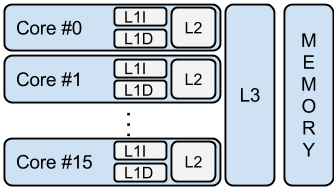
\includegraphics[scale=.65]{figures/processor_model/processor_model}
\caption{Generic Chip Multiprocessor Architecture.}
\label{fig:cmp_model}
\end{figure}

Memory is a vital component of any computing system, without memory we are unable to store our programs and computations.
Traditionally the technology used to create memories have differed from the technology used in processors~\cite{Wilkes2001}.
As processor performance increased, memory performance did not increase proportionally.
This development has resulted in what is known as the processor-memory gap~\cite{Wilkes2001}.
In order to mitigate this effect, small and fast memory structures known as caches are a vital part of both single core processors and CMPs.
Any memory request issued by a processing core is filtered through one or multiple caches before being issued to the main memory.
If any of the caches has the value of the requested memory address, the value is returned, and the memory request never reaches the main memory.
This mechanism to an extent can hide the processor-memory gap, given a high hit rate in cache memories.

\begin{figure}
    \centering
    \begin{subfigure}[b]{0.48\textwidth}
        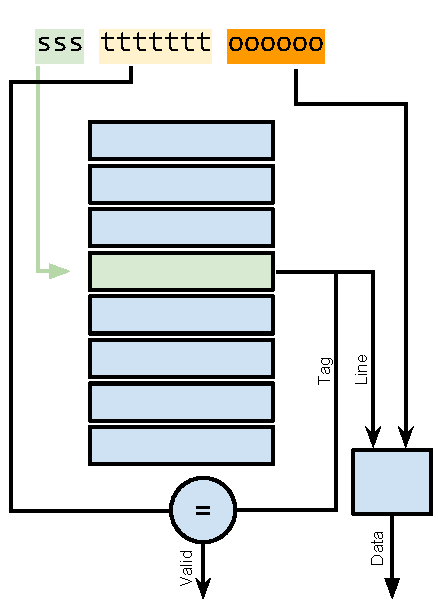
\includegraphics[width=\textwidth]{figures/introduction/dircache_read}
        \caption{Direct mapped cache. Each set contains only one block. The three most significant bits used for set addressing.}
        \label{fig:introduction:cache:dir}
    \end{subfigure}\hfill%
    \begin{subfigure}[b]{0.48\textwidth}
        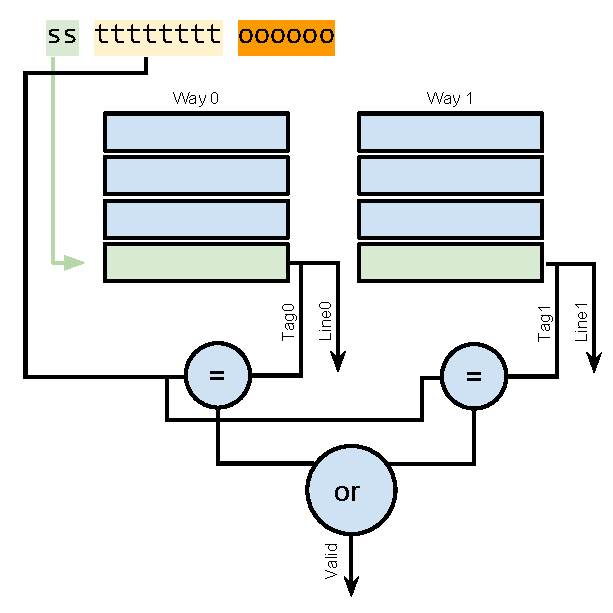
\includegraphics[width=\textwidth]{figures/introduction/2waycache_read}
        \caption{2-way associative cache. A selector, not shown here, is used to select between line0 and line1 to produce the data output. Each set contain two blocks, and compared to the direct case, additional hardware is required to select the correct output. Two bits used to set addressing, the most significant bit ignored.}
        \label{fig:introduction:cache:2way}
    \end{subfigure}
    \caption{Simplified architecture of a direct and 2-way cache under a read operation. With 64B lines, 7-bit tags, and byte addressing.}
    \label{fig:introduction:cache}
\end{figure}

Traditionally there are three main ways of organizing cache memory; direct, set-associative and fully associative.
Caches used in commercial CMPs today are set associative memory structures~\cite{Thomadakis2011, Jain2013, ARM2010, Ho2014}.
A cache is organized a 2d array, where each row is called a set, and each set consist of one or more blocks, sometimes known as cache lines.
A block is the minimum unit of data a cache stores, this is typically 64B.
The cache divides all memory addresses into three portions, the set address, block tag and block offset.
The set address is used to determine which set is responsible for caching a value.
Within a set, all blocks are valid cache locations.
Each block that contains valid data also stores the block tag of the data it contains.
During a cache lookup, all valid blocks will be scanned looking for one containing the block tag from the address.
In a direct mapped cache, each set contains only one block, making the block scan cheap.
Fully associative caches have all blocks in a single set, and the block scan is expensive in this case.
Set associative caches, also known as n-way caches, is a middle ground organization that stores n blocks per set.
Figure~\ref{fig:introduction:cache} shows both a direct and a 2-way cache under a read operation.
The figure does not show a fully associative cache organization, but its organization is deductible from the 2-way cache organization.
In this thesis, we will show that increasing the number of ways can improve performance of a cache and the cache partitioning algorithms.
However, from this architectural overview it is apparent that the critical path and complexity of a cache also increases as the number of ways increases.
As a result, first level caches are often limited to 2- or 4-ways~\cite{Sanchez2010}, because of the access latency must be short to prevent the CPU stalling while it waits for data. 
Even third level caches rarely exceed 16- or 32-ways.
There exists alternative cache organizations, such as zcache~\cite{Sanchez2010}, which allows for higher associativity at a lower cost.
These techniques are not currently used in commercial CMPs and hence are not considered further in this thesis.

When data not present in the cache is requested by a processing core, a request is sent the cache to the next cache level, or possibly the main memory.
Once the cache receives a response, it normally stores the data to provide faster access times in case of a re-reference.
Caches also normally store data that is written by a processing core, speeding up the write operation.
For a set-associative or fully associative cache, there are multiple valid storage positions for a data block.
It is the job of a cache partitioning algorithm to define which block is used to store the new data.
If the block selected is already in use, the cache removes, or evicts, the existing data.

In the memory hierarchy, smaller means faster. 
For instance, main memory is much faster than disks, but disks can store much more data.
The same is valid for caches, a smaller cache has a lower response time compared to a larger cache.
Figure~\ref{fig:cmp_model} shows an example 16-core CMP architecture with three cache levels and main memory.
For each cache level, the size increased and response time decreases.
The first level caches are the smallest while the third level caches are largest.
In order to save area on CMP chips, and also to provide an easy mechanism for data sharing between cores, it is common to have at least one level of shared cache.
In figure~\ref{fig:cmp_model} each core has a private L1 and L2 cache, and a shared last-level cache (LLC), the L3 cache.
While sharing cache can improve performance, and improve overall utilization, it also makes the memory system exposed to destructive interference that potentially can hurt the performance of all processing cores. 
The cache partitioning algorithm, running on the shared cache, may either ignore the effects of interference or it may attempt to reduce it by some form of prioritization.


\section{Requirements and Contributions}
By analyzing the problem description, we have been able to extract a set of requirements that this thesis has to fulfill:

\begin{description}
    \item[R1] Introduce CMPs, their memory system, and the role of a cache partitioning algorithm.
    \item[R2] Present important and recent work in the cache partitioning field. Present their strength and weaknesses, and compare them based on expected performance and overhead.
    \item[R3] Create a framework for evaluation of various cache partitioning algorithms.
    \item[R4] Implement at least one of the presented algorithm and compare against a conventional LRU-managed cache.
\end{description}

Based on the second requirement, this thesis will include a curated list of cache partitioning algorithms selected for their importance or recency in the field.
Due to the amount of work in this field we have to select some properties that each algorithm must have in order to appear in our list of algorithms.
Each algorithm will be presented in detail at a theoretical level, with comparisons to other relevant algorithms.

To fulfill the third and fourth requirement, we will implement a simulation framework and within that framework implement several of the algorithms selected.
We present a series of experiments executed on this implementation.
The resulting data will be used to compare the various algorithms against each other, providing depth to the theoretical comparison.
In addition, an evaluation of the implemented simulation framework will be performed.
This evaluation will explore the validity of our results.
The implemented simulation framework will at the end of this thesis be made available to NTNU and the CARD~\cite{CARD2015} research group for future research.

\section{Outline}

Chapter~\ref{cpt:introduction} introduces the thesis by putting it in a historical context and presenting the contributions made, fulfilling requirement \textbf{R1}.

Chapter~\ref{cpt:algorithms} presents a selection of cache partitioning algorithms and provides a theoretical comparison of them, fulfilling requirement \textbf{R2}.

Chapter~\ref{cpt:implementation} presents the subset of algorithms that we implement within our simulation framework.
Any assumptions or changes we have made compared to the theoretical description of the algorithm in chapter~\ref{cpt:algorithms} are presented here.

Chapter~\ref{cpt:methodology} contains a description of our simulation framework and explains all metrics we later use to evaluate our experiments, this fulfills requirement~\textbf{R3}.

Chapter~\ref{cpt:results} presents all experiments performed during the work with this thesis and evaluates their results. 
This evaluation includes a performance comparison of all implemented cache partitioning algorithms, fulfilling requirement \textbf{R4}.

Chapters~\ref{cpt:discussion} and~\ref{cpt:conclusion} contains a discussion of our results and a conclusion based on these. 
In addition, an overview of future work is given.